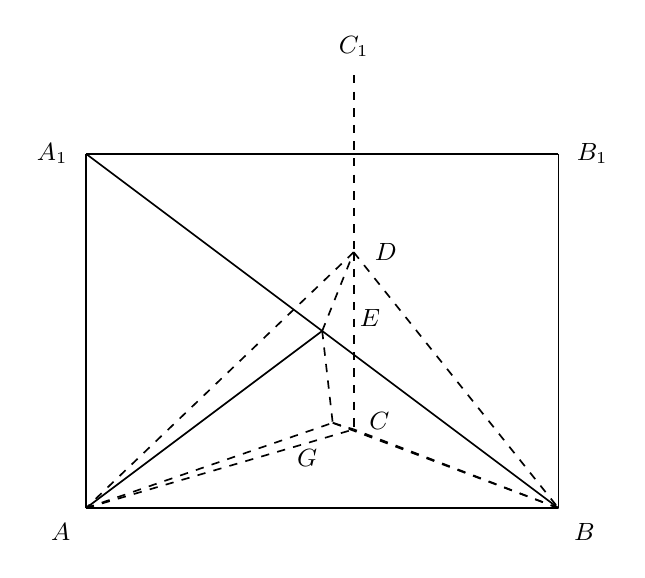
\begin{tikzpicture}[line width=0.6pt, font=\small]
\coordinate (A) at (0,0);
\coordinate (B) at (6,0);
\coordinate (C) at (3.4,1.0);
\coordinate (A1) at (0,4.5);
\coordinate (B1) at (6.0000000000,4.5000000000);
\coordinate (C1) at (3.4000000000,5.5000000000);
\coordinate (D) at (3.4000000000,3.2500000000);
\coordinate (E) at (3.0000000000,2.2500000000);
\coordinate (G) at (3.1333333333,1.0833333333);
% prism outline solid
\draw (A1)--(B1); \draw (A1)--(A); \draw (B1)--(B); \draw (A)--(B);
% hidden back edges dashed
\draw[dashed] (C1)--(D); \draw[dashed] (D)--(C);
\draw[dashed] (A)--(C); \draw[dashed] (B)--(C);
% diagonals
\draw (A1)--(B);
\draw (A)--(E); \draw[dashed] (E)--(D);
\draw[dashed] (D)--(B);
\draw[dashed] (D)--(A);
\draw[dashed] (E)--(G); \draw[dashed] (A)--(G); \draw[dashed] (G)--(C); \draw[dashed] (B)--(G);
% labels offset to avoid strokes
\node[left=3pt] at (A1) {$A_{1}$};
\node[right=3pt] at (B1) {$B_{1}$};
\node[above=3pt] at (C1) {$C_{1}$};
\node[below left=2pt] at (A) {$A$};
\node[below right=2pt] at (B) {$B$};
\node[right=3pt,xshift=-1pt,yshift=3pt] at (C) {$C$};
\node[right=4pt] at (D) {$D$};
\node[above right=3pt,xshift=7pt,yshift=-5pt] at (E) {$E$};
\node[below left=3pt,xshift=1pt,yshift=-3pt] at (G) {$G$};
\end{tikzpicture}
